\documentclass[handout]{beamer}

\usepackage{amsmath,amssymb,amsfonts,bm,dcolumn,color,graphicx,graphics,setspace,latexsym,setspace,lscape,subfigure,placeins,epsfig,hyperref}
\usepackage{eulervm}

% \usetheme{lucid}
% \usetheme{Madrid}
\definecolor{gray}{RGB}{30,30,30}
\definecolor{focus-fg}{RGB}{54,144,50}
\definecolor{lucid-blue}{RGB}{41, 170, 225}
\definecolor{light-grey}{RGB}{212, 212, 212}

\usepackage{tikz, tikz-cd, pgfplots}
\usetikzlibrary {arrows.meta,backgrounds,fit,positioning,petri}

\title{Deep Learning in Ecology}
\subtitle{Appling for a postdoc position within QBD}
% \author{Anonumous}
% \institute{Overleaf}
\date{\today}

\begin{document}

\frame{\titlepage}

\begin{frame}
    \frametitle{Table of Contents}
    \tableofcontents
\end{frame}

\section{Introduction}

\frame{
    \frametitle{Background}
    \begin{columns}[T]
        \begin{column}{5cm}
            \includegraphics[height=6.5cm]{family-photo.jpg}            
        \end{column}
        \begin{column}{6cm}
            \begin{itemize}
                \item In Ecology: Stability and structure of networked ecological systems
                \begin{itemize}
                    \item Scientific Reports, Journal of Biological Theory
                \end{itemize}
                \item In Machine Learning: Python-based deep learning frameworks such as Pytorch and jax. Github homepage https://github.com/keepsimpler/
            \end{itemize}
        \end{column}
    \end{columns}
}

\section{Deep Learning in Ecology}

\frame{
    \frametitle{Model}
    \framesubtitle{Concepts}
    Species is affected by its environment and other species around it.
    \vfill
    \centering
    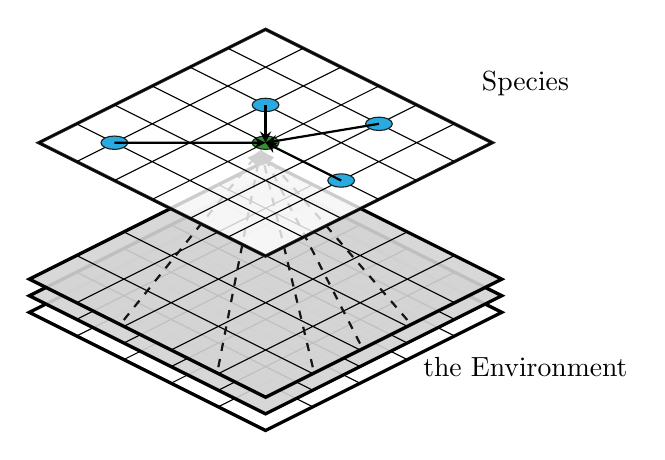
\begin{tikzpicture}[scale=.6,every node/.style={minimum size=1cm},on grid]
        \begin{scope}[
                yshift=-95,every node/.append style={
                yslant=0.5,xslant=-1},yslant=0.5,xslant=-1
                ]
            \fill[white,fill opacity=0.9] (0,0) rectangle (5,5);
            \draw[step=10mm, black] (0,0) grid (5,5);
            \draw[black,very thick] (0,0) rectangle (5,5);
        \end{scope}
        \begin{scope}[
                yshift=-85,every node/.append style={
                yslant=0.5,xslant=-1},yslant=0.5,xslant=-1
                ]
            \fill[light-grey,fill opacity=0.9] (0,0) rectangle (5,5);
            \draw[step=10mm, black] (0,0) grid (5,5);
            \draw[black,very thick] (0,0) rectangle (5,5);
        \end{scope}
        \begin{scope}[
            yshift=-75,every node/.append style={
            yslant=0.5,xslant=-1},yslant=0.5,xslant=-1
            ]
        \fill[light-grey,fill opacity=0.9] (0,0) rectangle (5,5);
        \draw[step=10mm, black] (0,0) grid (5,5);
        \draw[black,very thick] (0,0) rectangle (5,5);
    \end{scope}
        \draw[-latex,thick,gray!70!black, dashed](-1,-2) -- (-0.1,2.6);
        \draw[-latex,thick,gray!70!black, dashed](-3,-1) -- (-0.1,2.6);
        \draw[-latex,thick,gray!70!black, dashed](1,-2) -- (-0.1,2.6);
        \draw[-latex,thick,gray!70!black, dashed](2,-1.5) -- (-0.1,2.6);
        \draw[-latex,thick,gray!70!black, dashed](3,-1) -- (-0.1,2.6);
    \begin{scope}[
            yshift=10,every node/.append style={
            yslant=0.5,xslant=-1},yslant=0.5,xslant=-1
            ]
        \fill[white,fill opacity=0.8] (0,0) rectangle (4.8,4.8);
        \draw[gray,very thick] (0,0) rectangle (4.8,4.8);
        \draw[step=8mm, black] (0,0) grid (4.8,4.8);
        \draw [gray,fill=focus-fg] (2.4,2.4) circle [radius=0.2]; %
        \draw [gray,fill=lucid-blue] (0.8,4.0) circle [radius=0.2]; %
        \draw [gray,fill=lucid-blue] (2.4,0.8) circle [radius=0.2]; %
        \draw [gray,fill=lucid-blue] (3.2,3.2) circle [radius=0.2]; %
        \draw [gray,fill=lucid-blue] (4.0,1.6) circle [radius=0.2]; %
        \draw[thick, black, -stealth] (0.8,4.0) -- (2.4,2.4);
        \draw[thick, black, -stealth] (2.4,0.8) -- (2.4,2.4);
        \draw[thick, black, -stealth] (3.2,3.2) -- (2.4,2.4);
        \draw[thick, black, -stealth] (4.0,1.6) -- (2.4,2.4);
        \end{scope}
    %
    %
        \draw[thick](5.5,4) node {Species};
    %
        \draw[thick](5.5,-2) node {the Environment};
    %
    \end{tikzpicture}}

\frame{
    \frametitle{Model}
    \framesubtitle{Equation}
    Predict the probability of the presence of all the possible species at given locations according to the observed species occurrence data and environmental data:
    \begin{equation} \nonumber
        p(\bm{y}|\bm{x},\bm{z}) = f(\bm{x},\bm{z})
    \end{equation}
    Where:
    \begin{itemize} %[<+->]
        \item $\bm{y}$ is a random variable that can take on one of $S$ possible species
        \item $\bm{x}$ is the observed species occurrence data
        \item $\bm{z}$ is the observed environmental data
    \end{itemize}
}

\begin{frame}[t]
    \frametitle{Model}
    \framesubtitle{Training Steps}
    For any target species $s$ at a location, we:
    \begin{enumerate}
        \item find all the species and the environmental data that are within a distance (such as 10km) to the target species. 
        \item embed or project the above data into a latent space.
        \item learn the representation of the species niches using the state-of-art architecture such as Transformer.
        \item map the representation back to a categorical distribution on $S$ possible species.
        \item use a cross entropy loss between the categorical distribution and the target species to optimize.
    \end{enumerate}
    % We repeat the above procedure until loss does not decrease. At validate or test time, we
\end{frame}

\frame[t]{
    \frametitle{Model}
    \framesubtitle{Deep Neural Network Architecture}
    \vspace{0.2cm}
    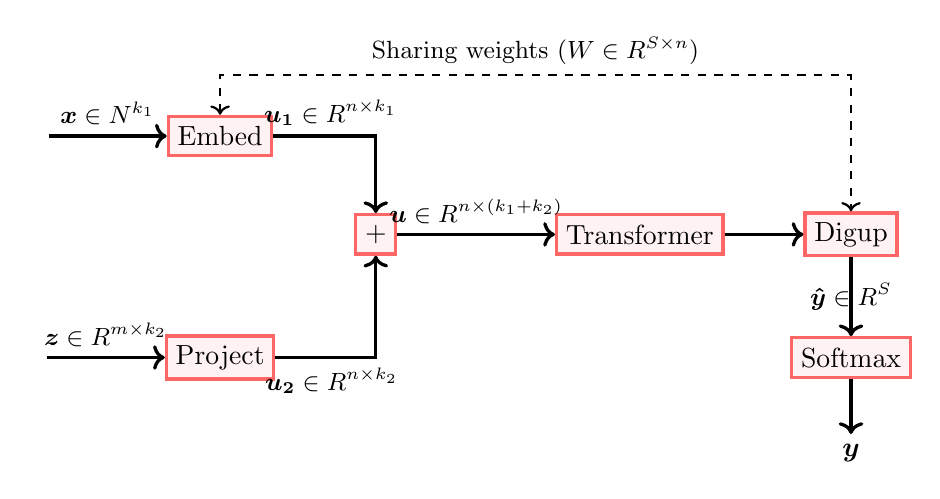
\begin{tikzpicture}[
        DLE/.style={rectangle, draw=red!60, fill=red!5, very thick, minimum size=5mm},  % Deep Learning in Ecology
    ]
        %Nodes
        \node (X) {};
        \node[DLE] (Embed) [right=1.5cm of X] {Embed};
        % \node (EmbedW) [below=0.cm of Embed] {\small $W \in R^{S \times n}$};
        \node (Dummy) [below=of Embed] {};
        \node[DLE] (Project) [below=of Dummy] {Project};
        \node (Z) [left=1.5cm of Project] {};
        \node[DLE] (Concat) [above right=of Project] {$+$};
        \node[DLE] (Transformer) [right= 2cm of Concat] {Transformer};
        \node[DLE] (Digup) [right=of Transformer] {Digup};
        \node[DLE] (Softmax) [below=of Digup] {Softmax};
        \node (Y) [below=0.7cm of Softmax] {$\bm{y}$};

        %Lines
        \draw[->, very thick] (X.east) to node[above] {\small $\bm{x} \in N^{k_1}$} (Embed.west);
        \draw[->, very thick] (Z.east) to node[above] {\small $\bm{z} \in R^{m \times k_2}$} (Project.west);
        \draw[->, very thick] (Embed.east) -| node[above, pos=0.28] {\small $\bm{u_1} \in R^{n \times k_1}$} (Concat.north);
        \draw[->, very thick] (Project.east) -| node[below, pos=0.28] {\small $\bm{u_2} \in R^{n \times k_2}$} (Concat.south);
        \draw[->, very thick] (Concat.east) to node[above] {\small $\bm{u} \in R^{n \times (k_1+k_2)}$} (Transformer.west);
        \draw[->, very thick] (Transformer.east) to (Digup.west);
        \draw[->, very thick] (Digup.south) to node {\small $\bm{\hat{y}} \in R^S$} (Softmax.north);
        \draw[->, very thick] (Softmax.south) to (Y.north);
        \draw[<->, dashed, thick] (Embed.north) -- +(0,0.5cm) -| node[above, pos=0.25] {\small Sharing weights ($W \in R^{S \times n}$)} (Digup.north);
    \end{tikzpicture}
    % $k_1$ is the number of all neighbor species, $\bm{x} \in N^{k_1}$ are all the neighbor species.
    % $k_2$ is the number of all the neighbor locations where environmental data are observed, $\bm{z} \in R^{m \times k_2}$ are the environmental data, where $m$ is the observed environment predictors at each observing point.
    % 
}


\frame{
    \frametitle{Data}
    \framesubtitle<>{GBIF Species Occurrence Data}
    \begin{columns}[c]
        \begin{column}{8cm}
            \includegraphics[height=6cm]{gbif_nl_stats.PNG}            
        \end{column}
        \begin{column}{3cm}
            \Huge \alert<>{1,356,807 \\ samples}
        \end{column}
    \end{columns}
}

\frame[t]{
    \frametitle{Data}
    \begin{block}{GBIF Species Occurrence Data}
    \end{block}
    \begin{columns}[t]
        \begin{column}{6cm}
            Species distribution
            \includegraphics[height=4.5cm]{species_distribution.png}            
        \end{column}
        \begin{column}{4cm}
            Top10 species and \\ their counts:
            \includegraphics[height=4.5cm]{top_10_species.PNG}            
        \end{column}
    \end{columns}
}

\frame[t]{
    \frametitle{Data}
    \begin{block}{WorldClim Historical Climate Data}
    \end{block}
    \begin{columns}[T]
        \begin{column}{7cm}
            \includegraphics[height=7cm]{bio_1_19.png}            
        \end{column}
        \begin{column}{4.5cm}
            \centering
            Bioclimatic variables
            \tiny
            \begin{table}[]
                \begin{tabular}{l|l}
                \hline
                BIO1  & Annual Mean Temperature \\ \hline
                BIO2  & Mean Diurnal Range \\ \hline
                BIO3  & Isothermality (BIO2/BIO7) \\ \hline
                BIO4  & Temperature Seasonality \\ \hline
                BIO5  & Max Temperature of Warmest Month \\ \hline
                BIO6  & Min Temperature of Coldest Month \\ \hline
                BIO7  & Temperature Annual Range \\ \hline
                BIO8  & Mean Temperature of Wettest Quarter \\ \hline
                BIO9  & Mean Temperature of Driest Quarter \\ \hline
                BIO10 & Mean Temperature of Warmest Quarter \\ \hline
                BIO11 & Mean Temperature of Coldest Quarter \\ \hline
                BIO12 & Annual Precipitation \\ \hline
                BIO13 & Precipitation of Wettest Month \\ \hline
                BIO14 & Precipitation of Driest Month \\ \hline
                BIO15 & Precipitation Seasonality\\ \hline
                BIO16 & Precipitation of Wettest Quarter \\ \hline
                BIO17 & Precipitation of Driest Quarter \\ \hline
                BIO18 & Precipitation of Warmest Quarter\\ \hline
                BIO19 & Precipitation of Coldest Quarter \\ \hline
                \end{tabular}
            \end{table}
        \end{column}
    \end{columns}
}

\begin{frame}[t]
    \frametitle{Explainable NN Model}
    \framesubtitle{Quantitative Niche Modeling}
    \begin{itemize}
        \item The feature vector of a species in the latent space works as its quantitative niche. 
        \item The cosine similarity among feature vectors explain the relationship among the corresponding species.  % which is analog to the embedding vectors of words in language models
    \end{itemize}
    \vspace{0.2cm}
    \begin{tikzpicture}
        \node[inner sep=0pt] (Features) at (4,0)
        {\includegraphics[width=.7\textwidth]{feature_vectors.PNG}};
        \node[left] (Species1) at (0,2.1) {\tiny Gasterosteus aculeatus};
        \node[left] (Species2) at (0,1.5) {\tiny Gallinula chloropus};
        \node[left] (Species3) at (0,0.9) {\tiny Hydriomena impluviata};
        \node[left] (Species4) at (0,0.3) {\tiny Elophila nymphaeata};
        \node[left] (Species5) at (0,-0.3) {\tiny Ameiurus nebulosus};
        \node[left] (Species6) at (0,-0.9) {\tiny Colias hyale};
        \node[left] (Species7) at (0,-1.5) {\tiny Scotopteryx chenopodiata};
        \node[left] (Species8) at (0,-2.1) {\tiny Epermenia illigerella};
    \end{tikzpicture}    
\end{frame}

\begin{frame}[t]
    \frametitle{Explainable NN Model}
    \framesubtitle{Saliency maps}
    The derivatives of a species $i$'s occurrence probability $p(\bm{y}_i)$ with respect to the environmental data and the species occurrence data:

    \begin{equation}
        \frac{\text{d}p(\bm{y}_i|\bm{x},\bm{z})}{\text{d} \bm{z}}
    \end{equation}
    \begin{equation}
        \frac{\text{d}p(\bm{y}_i|\bm{x},\bm{z})}{\text{d} \bm{x}}   
    \end{equation}
    % \begin{tikzpicture}
    %     \node[inner sep=0pt] (Features) at (0,0)
    %     {\includegraphics[width=.3\textwidth]{bio_1_19.png}};
    % \end{tikzpicture}    
    
\end{frame}


\begin{frame}[t]
    \frametitle{Future works}
    \framesubtitle{}
    \begin{enumerate}
        \item Explore the explainable model.
        \item Add Time Dimension for the species occurrence data and the environment data.
        \item Hierarchical in taxonomic: kingdom, phylum, class, order, family, genus and species.
        \item Predict the rare species
    \end{enumerate}
    
\end{frame}


\end{document}